\subsection{Overview and Conceptual Framework}
\label{principles-overview}

After the goal of manifold learning has been formalized, it shall now be laid 
out how the problem is approached by LLE as the conceptual parent of SS-LLE 
The incorporation of prior information is a rather different matter that will be 
addressed in chapter \ref{sslle}. 
Much of the theoretical foundation for LLE has been discussed only in later 
work.
In order to provide a more integrated background, explanations will therefore be 
given in a broader context of local graph-based manifold learning which also 
comprises Laplacian eigenmaps and H-LLE.
The particular relationship of the three methods shall be made clear along the 
way.

Local graph-based manifold learning generally arises from a variety 
of geometric intuitions and computational implementations.
Nonetheless, methods share common structures that allow for interpretation in a 
more abstract framework (\citet{bengioetal2003}, \citet{bengioetal2004}).
It should be noted that such a framework might be established from several 
perspectives; after all, the different methods attempt to solve the same problem 
and can thus often be translated into one another.
This report will sketch the idea behind local graph-based manifold learning in 
the light of \textit{kernel principal component analysis (kernel PCA)}.
The reasoning behind this choice is that kernel PCA provides a useful 
intuition to manifold learning and subsumes the other methods in a way that 
proves beneficial for out-of-sample extension \citep{bengioetal2004}.
Kernel PCA was actually proposed first and later shown to link the others by a 
unified idea (\citet{hametal2003}, \citet{bengioetal2004}). 

\begin{center}
  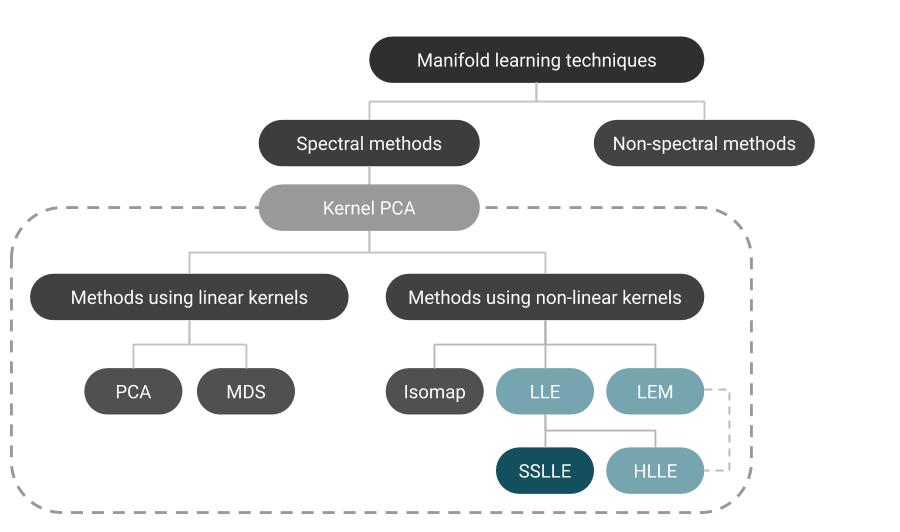
\includegraphics[width = 0.8\textwidth]{figures/models-overview}
\end{center}

Tree plot with models
Kernel PCA
Non-linearity + corresponding graph structure
Locality

% ------------------------------------------------------------------------------

\subsection{Unsupervised Techniques}
\label{techniques}

% ------------------------------------------------------------------------------

\subsubsection{Laplacian Eigenmaps}
\label{laplace}

\begin{itemize}
  \item Notion of locality
  \item Laplacian eigenmaps
\end{itemize}

% ------------------------------------------------------------------------------

\subsubsection{Locally Linear Embedding (LLE)}
\label{lle}

\begin{itemize}
  \item Notion of local linearity
  \item Approximation of graph Laplacian
\end{itemize}

% TODO Regularized version???

% ------------------------------------------------------------------------------

\subsubsection{Hessian Locally Linear Embedding (H-LLE)}
\label{hlle}

\begin{itemize}
  \item Hessian instead of Laplacian (eigenmaps)
  \item Hessian instead of LS fit (LLE)
\end{itemize}
